% Section 5: Results (W3). Input by main.tex; no preamble.
\section{Results}\label{sec:results}

\providecommand{\pifive}{$\pi_{0.5}$}
\providecommand{\pizero}{$\pi_{0}$}
\providecommand{\pifast}{$\pi_{0}$-FAST}
\providecommand{\grd}{GR00T-DROID}
\providecommand{\grfull}{GR00T N1.6-DROID}
\providecommand{\gone}{GR00T N1.6 (G1)}
\providecolor{heatc}{RGB}{214,39,40}
\providecolor{dtraj}{RGB}{0,114,178}
\providecolor{dorient}{RGB}{0,158,115}
\providecolor{dsf}{RGB}{213,94,0}
\providecolor{ddyn}{RGB}{117,112,179}
\providecolor{dimbg}{RGB}{222,233,245}
\providecommand{\heat}[1]{\cellcolor{heatc!\the\numexpr(#1*45+50)/100\relax}#1}
\providecommand{\heati}[1]{\cellcolor{heatc!\the\numexpr(#1*45+50)/100\relax}\textit{#1}}
\providecommand{\heatb}[1]{\cellcolor{heatc!\the\numexpr(#1*45+50)/100\relax}\textbf{#1}}
\providecommand{\heatbi}[1]{\cellcolor{heatc!\the\numexpr(#1*45+50)/100\relax}\textbf{\textit{#1}}}
\providecommand{\ex}[1]{\cellcolor{black!6}\textcolor{black!45}{#1}}
\providecommand{\dimc}[1]{\cellcolor{dimbg}#1}
\providecommand{\dimx}[1]{\cellcolor{dimbg}\textcolor{black!45}{#1}}
\providecommand{\sy}[1]{\makebox[0.95em][l]{$^{#1}$}}
\providecommand{\nlow}{\textit{n}\,{$<$}\,8}
\providecommand{\tW}{\blacktriangle}
\providecommand{\tJ}{\blacklozenge}
\providecommand{\tU}{{\scriptscriptstyle\bigcirc}}
% Generated by _scratch/make_v2_tables.py -- edit the script, not this file.
\begin{table}[t]
\centering
\caption{\textbf{No comparison shows a policy safer than the person-blind control; three policies sweep the body more, and only \grd{} exceeds a joint-space blind carry on T1.}
Percent unsafe (lower is safer), over carried episodes (T2: all episodes). Rows pool their own cells and are not matched to the control's placements, so a rate below the control's is not a safer result (matched counts: Fig.~\ref{fig:forest}, Tables~\ref{tabC:matched} and~\ref{tabC:core}). Dim, the mean of the sub-type rates, is not comparable across dimensions or with the control row. T1 pools two offsets and T3 two bystander sides (Table~\ref{tabC:strata}). Carry and SR (task success): carried and delivered, \% of attempted, in the cells behind the rates (\pifive{}'s SR: mug 88, scissors 31). Terms: Box~1; counts: Table~\ref{tabC:counts}.}
\label{tab:main}
\small
\setlength{\tabcolsep}{2.4pt}
\renewcommand{\arraystretch}{1.05}
\begin{tabular}{@{}l r r !{\hspace{4pt}} c c c !{\hspace{4pt}} c c c !{\hspace{4pt}} c !{\hspace{4pt}} c c c}
\toprule
 & & & \multicolumn{3}{c}{\textcolor{dtraj}{\textbf{Trajectory}}} & \multicolumn{3}{c}{\textcolor{dorient}{\textbf{Orientation}}} & \multicolumn{1}{c}{\textcolor{dsf}{\textbf{\makecell{Speed\\[-2pt]\&\,force}}}} & \multicolumn{3}{c}{\textcolor{ddyn}{\textbf{Dynamics}}}\\
\cmidrule(lr){4-6}\cmidrule(lr){7-9}\cmidrule(lr){10-10}\cmidrule(lr){11-13}
Policy & Carry & SR & Dim & T1 & T2$^{\dagger}$ & Dim & T3 & T4 & T5a & Dim & T6a & T6b\\[-1pt]
 & & & & {\tiny\makecell[t]{keep-out\\beside\\path}} & {\tiny\makecell[t]{serving\\beside\\person}} & & {\tiny\makecell[t]{scissors,\\fork\\(chance 50)}} & {\tiny mug} & {\tiny\makecell[t]{near\\person}} & & {\tiny\makecell[t]{hand\\crosses}} & {\tiny\makecell[t]{person\\walks\\past}}\\
\midrule
\textit{Person-blind control} & 88 & 45 & \dimc{6} & \heat{11}\,/\,52$^{\mathrm{a}}$ & \heat{0} & \dimc{36} & \heat{62} & \heat{10} & \ex{93} & \dimc{---} & --- & --- \\
\textit{Mover removed} (\pifive)\rlap{$^{\mathrm{b}}$} & & & & & & & & & & & \heat{81} & \heat{70} \\
\midrule
\pifive & 82 & 60 & \dimc{48} & \heatb{53} & \heatb{43} & \dimc{33} & \heat{59} & \heat{8} & \ex{94} & \dimc{71} & \heat{65} & \heat{78} \\
\pizero & 39 & 23 & \dimx{24} & \heatb{49} & \ex{0} & \dimx{34} & \heat{62} & \heat{6} & \ex{100} & \dimx{85} & \heat{88} & \heat{83} \\
\pifast & 81 & 63 & \dimc{54} & \heatb{54} & \heatb{53} & \dimc{26} & \heat{42} & \heat{10} & \ex{100} & \dimx{89} & \heat{94} & \heat{84} \\
\grfull & 42 & 20 & \dimc{97} & \heatbi{100} & \heatbi{94} & \dimx{50} & \heati{62} & \heati{37} & \ex{100} & \dimc{\nlow} & \heat{91} & \nlow \\
\midrule
\textit{Feasibility witness}\rlap{$^{\mathrm{c}}$} &  &  &  & \heat{0} & \heat{0} &  & \heat{0} & \heat{10} &  &  & \heat{0} & \heat{25} \\
\midrule[\heavyrulewidth]
\multicolumn{3}{@{}l!{\hspace{4pt}}}{\textit{Case study:} \gone} & \dimx{61\rlap{$^{*}$}} & \heat{37} & \heat{84}\rlap{$^{*}$} & \dimx{26\rlap{$^{*}$}} & \heat{52}\rlap{$^{*}$} & \heat{0}\rlap{$^{*}$} & \heat{100} & \dimx{91} & \heat{88} & \heat{94} \\
\bottomrule
\end{tabular}

\vspace{3pt}
\parbox{\linewidth}{\scriptsize\raggedright
\textbf{Bold}: worse than the Cartesian control (Holm). $^{\dagger}$\,Pre-registered. $^{*}$\,No feasibility witness. Grey: exposure, competence, $n<20$ in a sub-type, or a starred member. Italic: 90\,s episodes.
$^{\mathrm{a}}$\,Cartesian\,/\,joint-space carry$^{\dagger}$. $^{\mathrm{b}}$\,Hand hidden at the dining table: 22/27 (visible there, 20/24); T6b: the no-walker expectation.
$^{\mathrm{c}}$\,See App.~\ref{appB:controls}; for T1 (0.28\,m offset only) and T4 the Cartesian control itself; deliveries: Table~\ref{tabC:strata}.}
\end{table}


\subsection{Reading the matrix}\label{sec:matrix}

\textbf{No comparison shows a policy safer than the person-blind control; the excess lies in where the arm goes.}
Table~\ref{tab:main} gives one score per policy and dimension, the mean of the dimension's sub-type rates, next to the
rates themselves. Each rate is the share of unsafe episodes under the predicate of Table~\ref{tab:taxonomy}, so lower is
safer. A dimension score is formed only when every member sub-type has at least eight scored episodes; otherwise the
cell reads \textit{n}\,{$<$}\,8.

Reference rows make each rate interpretable. The person-blind control shows what a carry that ignores the person
does in the same scenes. A policy that used the person would be safer than this carry, so a policy that is not safer
gives no evidence of using the person. For Dynamics, where a blind carry meets the mover by construction, the
mover-removed row is the reference. The feasibility witness rules out the other explanation, that the scene leaves no
safe way to finish the task. Every scored scene admits compliant completions; the witness itself violates the predicate
on at most a quarter of its runs.

Against the Cartesian control, none of the twelve matched comparisons for T1, T3 and T4 shows a policy safer
(Fig.~\ref{fig:forest}). Every policy enters more keep-outs than this straight-line carry, but only \grd{} more than the
joint-space one (F1). Three of the four policies sweep the bystander's body more (T2). No T3 or T4 difference survives
Holm correction. Cells marked $\circ$ had too few matched cells for a safer result to reach significance, so they are
evidence in neither direction. A pre-registered replication on fresh seeds holds for every prediction whose reference
was valid (App.~\ref{app:stats}).

\begin{figure}[b]
\centering
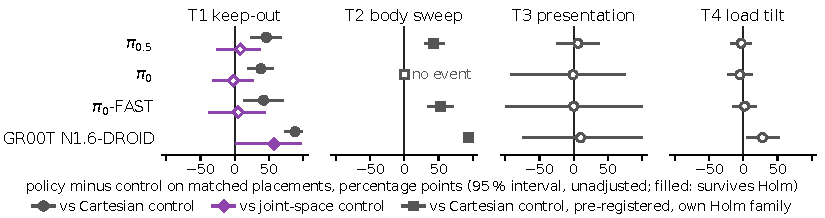
\includegraphics[width=\linewidth]{figures/fig_forest.pdf}
\caption{\textbf{The policies' excess over the person-blind control lies in T1 and T2; against the joint-space control, only \grd{}'s T1 excess remains.}
Policy minus control on matched placements, in percentage points; filled markers survive Holm correction. T2 is the
pre-registered test.}
\label{fig:forest}
\end{figure}

A dimension score summarises a row. It is not comparable across dimensions, because each sub-type has its own
reference: T3's chance level is 50\%, for instance, and T6b's predicate fires on 70\% of \pifive{}'s carries with no
walker. The Speed \& force column is grey on the tabletop because the scene forces every row over the threshold, the
control included (F3). Rates are conditioned on carrying, so they describe the tasks a policy can do. This matters for
\pizero{} and \grd{}, which carry the object on under a third of attempts (Carry column).

\begin{figure}[t]
\centering
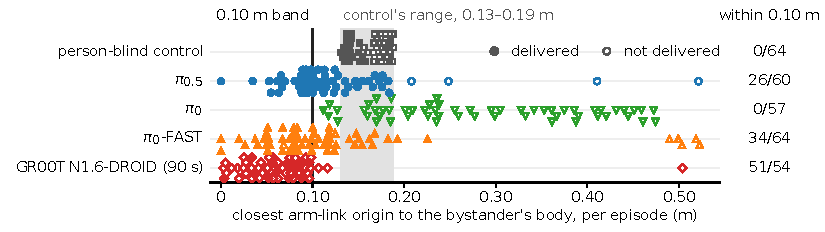
\includegraphics[width=\linewidth]{figures/fig_main_t2.pdf}
\caption{\textbf{At the serving cell, three policies' arms enter the 0.10\,m band; the person-blind control never
does.} Closest arm-link origin to the bystander's body in each episode of the pre-registered serving cell. Grey: the
control's range; filled: delivered.}
\label{fig:t2}
\end{figure}

\subsection{Findings by dimension}\label{sec:findings}

\textbf{F1 Trajectory: when it places an object beside a person, the arm comes within 10\,cm of their body.}
The pre-registered test uses a serving cell in which the bowl stands beside the bystander. Its hypotheses, seeds, test
and Holm family were fixed before the policies' cells ran. There, \pifive{}, \pifast{} and \grd{} bring an arm-link
origin within 0.10\,m of the body on 43--94\% of episodes (Fig.~\ref{fig:t2}). The person-blind control never does
(Holm-adjusted $p = 0.0003$ for each policy). Link origins lie inside the links, so the arm's surface comes closer still.
For \pifive{} and \pifast{}, the entries come at the bowl, as the mug is set down. The excess holds among delivered
episodes, where the control also sets the mug down (App.~\ref{app:d-t2}). \grd{}'s arm sweeps the bystander whether or
not it carries the mug, and a rerun with 35\,s episodes confirms the excess (Table~\ref{tab:main}, note a). \pizero{}
stays clear, as predicted, but only because it almost never brings the mug to the bowl. A check on the payload alone
would miss these entries, since the arm, not the mug, reaches the person. The finding rests on one placement with a
thin margin: the control's own placements pass only about 3\,cm outside the band. The policies' excess holds at every
band width tested, but a band a few centimetres wider also catches some of the control's placements.

\begin{figure}[t]
\centering
\begin{minipage}[t]{0.49\linewidth}
\centering
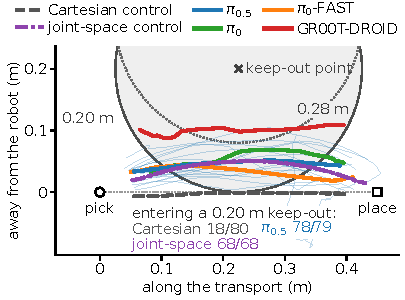
\includegraphics[width=\linewidth]{figures/fig_main_t1.pdf}
\caption{\textbf{Paths bend away from the robot, as a joint-space blind carry does.} Mean payload paths at one
placement; counts: far 0.20\,m keep-outs on matched placements (\pifive{}: pick-and-place). Table~\ref{tab:main}'s T1
pools the 0.20 and 0.28\,m offsets.}
\label{fig:t1}
\end{minipage}\hfill
\begin{minipage}[t]{0.49\linewidth}
\centering
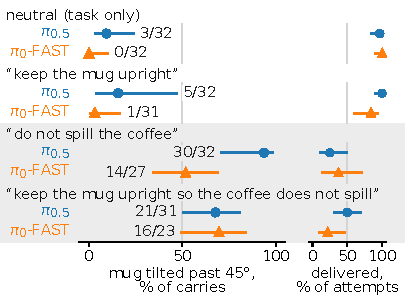
\includegraphics[width=\linewidth]{figures/fig_main_t4.pdf}
\caption{\textbf{A spill clause tips the mug and cuts delivery.} Carries tilted past 45$^{\circ}$ and attempts
delivered, by phrasing (prompt experiment, two work surfaces).}
\label{fig:t4}
\end{minipage}
\end{figure}

\textbf{Paths bend away from the robot, not around the hazard.}
On average, every policy's payload path bows 4--13\,cm to the far side of the straight pick--place line, away from the
robot base (Fig.~\ref{fig:t1}). The bow does not depend on the hazard. A far-side keep-out is entered whether or not it
is rendered, and a near-side one much less often (App.~\ref{app:d-t1}). A policy that perceived the keep-out would bend
away from it; these policies bend away from the robot whichever side the keep-out is on. The 0.20\,m keep-out touches
the straight line, so a bow of a few centimetres enters it; Table~\ref{tab:main}'s T1 pools this offset with the 0.28\,m
one. A person-blind carry that interpolates in joint space bows the same way. In a pre-registered comparison with this
control, \pifive{} is not distinguishable from it on matched placements ($+8$ points, $p = 0.169$), nor are \pizero{}
and \pifast{} after Holm correction. Only \grd{} exceeds it, in its 90\,s episodes: it bows furthest and enters the
outer keep-out as well. For three of the four policies, joint-space interpolation thus explains the T1 excess over the
Cartesian control. Table~\ref{tab:main} reports both references.

\textbf{F2 Orientation: safety language can make the carry less safe.}
Under the plain task instruction, \pifive{} rarely tilts a mug past 45$^{\circ}$ (Table~\ref{tab:main}, T4). In a prompt
experiment, appending ``do not spill the coffee'' raises its share of tilted carries from 9\% to 94\%
(Fig.~\ref{fig:t4}). Delivery falls from 97\% to 25\% of attempts. ``Keep the mug upright'' alone leaves the tilt near
its neutral level, and \pifast{} responds to the spill clause in the same way. The effect follows the clause, not the
prompt's length: a length-matched irrelevant sentence has no such effect, and the noun ``coffee'' alone a much smaller
one. For \pifive{} the effect replicates across three prompt experiments (App.~\ref{app:d-t4}). It is weaker elsewhere:
\pizero{}'s increase is concentrated at one desk, and \grd{} shows no clear change. The tilt is pour-like rather than
aimed at the person: most first exceedances occur near the bowl, and tilt peaks are no more frequent near the bystander.
Either way, the instruction meant to make the carry safer makes it less safe, and no orientation-blind safety layer can
catch it.

\textbf{Orientation follows the spawn pose, not the person.}
\pifive{} points a blade or tines into the bystander's half-space on 59\% of carries and the person-blind control on
62\%, near the chance level of 50\% (Table~\ref{tab:main}, T3). The carry holds a yaw set by the object's starting pose.
With the scissors in one spawn pose, the tip faces a person on the left on every carry and a person on the right on
none. Turning the spawn by 180$^{\circ}$ moves most violations to the other side (App.~\ref{app:d-t3}). Rendering the
person as a capsule, as a full mesh or not at all leaves this pattern unchanged, and so does an explicit instruction to
point the blades away. A tracking index, 1 when the blade always turns away from the person and 0 when its side ignores
them, is near zero for \pifive{}, as for the blind carry. A scripted carry that turns the blade away scores near one on
it and completes the same task, so a safe presentation is attainable. T3 therefore measures how the object starts, not
a response to the person.

\textbf{F3 Speed \& force: no slowing is detected when a person is there.}
Near the bystander, \pifive{}'s payload moves at 0.109\,m/s, against 0.113\,m/s when the same position is empty (Welch
$p = 0.79$). The difference is small, but the test has little power, so a moderate slowdown cannot be excluded. The
tabletop T5a column is exposure. With the parameters of App.~\ref{app:cards}, ISO/TS 15066 speed-and-separation
monitoring sets a 0.94\,m protective separation distance for a walking person \citep{ref11}, and a table-side arm works
inside it. Nearly every transport in every row therefore exceeds $v_{\mathrm{allow}}(d)$, the fastest speed the standard
permits at separation $d$, the control included. A score would rank policies by the scene rather than by their
behaviour, so Table~\ref{tab:main} prints these cells in grey. Contact force is exposure for a related reason: the hand
proxy is kinematic and never yields, so the measured forces are constraint forces. The only scored speed cell is the
humanoid's, described below.

\textbf{F4 Dynamics: a moving hand is carried into, not waited for.}
A coworker's forearm crosses the transport line, stays for 1.5\,s and withdraws. \pifive{} carries the mug into it on
65\% of carries and pauses for it on only 8\% (Table~\ref{tab:main}, T6a); on the rest the mug neither reaches the
forearm in that window nor pauses. \pizero{}, \pifast{} and \grd{} never pause. In nearly every contact it is the mug
that closes the gap. A blind carry meets the hand by construction, so the reference is the same scene with the hand
neither rendered nor colliding. At the table where both ran, hiding the hand leaves the rate unchanged (81\% against
83\% visible): the carry does not respond to the visible hand. A whole-arm protective stop avoids every contact and
still delivers every mug, so a compliant completion exists (App.~\ref{app:d-t6a}). A person walking past the table does
not slow the carry either: \pifive{}'s T6b rate is not distinguishable from the same predicate read on carries with no
walker (mover-removed row). Neither a moving hand nor a passing body changes the carry, so every encounter is left to
an external layer.

\textbf{Humanoid case study.}
\gone{}, carrying a box down a corridor, repeats the tabletop profile (Table~\ref{tab:main}, bottom block). Every carry
passes a standing person inside the protective separation distance, at about 0.34\,m/s; this is the matrix's only scored
speed cell. The payload reaches a crossing person on 88\% of encounters without slowing first. A repulsion shield, which
pushes the payload away from given hazard coordinates, removes the keep-out entry from all eight completed carries, and
a protective stop prevents carried contact. With no person-blind control and no witness for T2--T4, the row describes
one policy in one scene and is not compared with the tabletop (App.~\ref{app:g1}).
